\documentclass[conference,letterpaper]{IEEEtran}
\IEEEoverridecommandlockouts
% Toque MCIC sobre IEEEtran: solo color y diagramas. No cambia márgenes,
% fuentes, columnas ni tamaños de la plantilla IEEE.
% tectonic compila con XeTeX: Times New Roman (la de IEEE y la secundaria del manual UD)
% se lee de las fuentes del manual de marca; si no está, TeX Gyre Termes (clon de Times).
\usepackage{amsmath,amssymb}
\usepackage{newtxmath}
\usepackage{fontspec}
\providecommand{\UDmarca}{/Users/juferoga/repos/ud/maestria/mcic/.UniversidadDistrital-manual-marca}
\IfFileExists{\UDmarca/fuentes/times.ttf}{%
  \setmainfont{times.ttf}[Path=\UDmarca/fuentes/, BoldFont=timesbd.ttf,
    ItalicFont=timesi.ttf, BoldItalicFont=timesbi.ttf]}{%
  \setmainfont{texgyretermes}[Extension=.otf, UprightFont=*-regular, BoldFont=*-bold,
    ItalicFont=*-italic, BoldItalicFont=*-bolditalic]}
\setmonofont{texgyrecursor}[Extension=.otf, UprightFont=*-regular, BoldFont=*-bold, Scale=0.95]
\usepackage[spanish,es-noshorthands,es-tabla,es-nolists]{babel}
\usepackage{graphicx}
\usepackage{booktabs,tabularx,array,multirow}
\usepackage[table]{xcolor}
\usepackage{tikz}
\usetikzlibrary{positioning,arrows.meta,calc,fit}
\usepackage[hidelinks]{hyperref}
\usepackage{cite}
\usepackage{url}

% Paleta del manual de marca UD (design.md)
\definecolor{udazul}{HTML}{1291C0}
\definecolor{udazulosc}{HTML}{0C6F96}
\definecolor{uddorado}{HTML}{B49739}
\definecolor{udverde}{HTML}{00A859}
\definecolor{udplata}{HTML}{98999A}
\definecolor{udsable}{HTML}{373435}
\definecolor{udrojo}{HTML}{ED3237}

\hypersetup{colorlinks=true,linkcolor=udazulosc,citecolor=udazulosc,urlcolor=udazulosc}

% Bloques de la ecuación de búsqueda: el mismo color en ecuación, PRISMA y matriz.
\newcommand{\bloqueA}[1]{\textcolor{udazulosc}{#1}}
\newcommand{\bloqueB}[1]{\textcolor{uddorado!85!black}{#1}}
\newcommand{\bloqueC}[1]{\textcolor{udverde!80!black}{#1}}
\newcommand{\etiqueta}[2]{\tikz[baseline=(t.base)]\node[fill=#1,text=white,inner sep=1.6pt,
  rounded corners=1pt,font=\bfseries\scriptsize](t){#2};}

% Cabecera de tablas: filete azul y fila sombreada clara
\newcommand{\cabecera}{\rowcolor{udazul!12}}
\arrayrulecolor{udazulosc}

% Columnas de la matriz
\newcolumntype{L}[1]{>{\raggedright\arraybackslash}p{#1}}
\newcolumntype{Y}{>{\raggedright\arraybackslash}X}

\makeatletter
\providecommand{\filas}[1]{\@@input #1 }
\makeatother

% Marca de enfoque en la matriz (A..E)
\newcommand{\enf}[1]{\textcolor{udazulosc}{\bfseries #1}}

% Cajas del PRISMA
\tikzset{
  caja/.style={draw=udazulosc,line width=0.5pt,rounded corners=1.5pt,align=center,
    font=\scriptsize,inner sep=2.5pt,text width=#1},
  caja/.default=3.6cm,
  excl/.style={draw=udplata,line width=0.5pt,rounded corners=1.5pt,align=left,
    font=\scriptsize,inner sep=2.5pt,fill=udplata!8,text width=#1},
  excl/.default=2.75cm,
  fase/.style={fill=udazul,text=white,font=\bfseries\tiny,minimum width=0.42cm,
    rounded corners=1pt,inner sep=1pt},
  flecha/.style={-{Latex[length=1.6mm]},udsable,line width=0.5pt},
}
\newcolumntype{Y}{>{\raggedright\arraybackslash}X}

\makeatletter
\providecommand{\filas}[1]{\@@input #1 }
\makeatother


\newcommand{\pendiente}[1]{\textcolor{udrojo}{\textbf{[#1]}}}
% Generado por revision/generar_e1.py; no editar a mano.
\newcommand{\nArxivQuno}{35}
\newcommand{\nArxivQdos}{3}
\newcommand{\nArxivTotal}{38}
\newcommand{\nArxivDup}{0}
\newcommand{\nOaQuno}{162}
\newcommand{\nOaQdos}{33}
\newcommand{\nOaTotal}{195}
\newcommand{\nOaDup}{39}
\newcommand{\nDup}{39}
\newcommand{\nTamizados}{194}
\newcommand{\nExclTitulo}{147}
\newcommand{\nPasan}{47}
\newcommand{\nExclTexto}{10}
\newcommand{\nIncluidosBases}{37}
\newcommand{\nOtros}{21}
\newcommand{\nTotalIncluidos}{58}
\newcommand{\nMatriz}{16}
\newcommand{\nMatrizRecientes}{13}
\newcommand{\nRecientes}{49}
\newcommand{\nTextoCompleto}{35}
\newcommand{\nSoloResumen}{23}
\newcommand{\fechaConsulta}{2026-11-06}
\newcommand{\fechaConsultaOa}{2026-11-07}
\newcommand{\nIncluidosCitados}{31}
\newcommand{\nReferencias}{46}

% Generado por articulo/generar_cifras.py; no editar a mano.
\newcommand{\cifCommits}{612.811}
\newcommand{\cifDesarrollo}{558.438}
\newcommand{\cifPrueba}{54.373}
\newcommand{\cifPrevMin}{3{,}9\,\%}
\newcommand{\cifPrevMax}{4{,}5\,\%}
\newcommand{\cifPrevAnioVeintiseis}{\pendiente{dato de prueba retirado}}
\newcommand{\cifPositivosDesarrollo}{23.735}
\newcommand{\cifPositivosPrueba}{\pendiente{dato de prueba retirado}}
\newcommand{\cifCensurados}{26.133}
\newcommand{\cifAutores}{18.127}
\newcommand{\cifSubsistemas}{748}
\newcommand{\cifNVariables}{22}
\newcommand{\cifParesCherry}{2.305}
\newcommand{\cifFracCherry}{0{,}41\,\%}
\newcommand{\cifDiscCherry}{78}
\newcommand{\cifDiasCherry}{3}
\newcommand{\cifGenes}{150}
\newcommand{\cifGenesReales}{45}
\newcommand{\cifEvalAptitud}{11.280}
\newcommand{\cifFilasAptitud}{80.000}
\newcommand{\cifSegEntrenamiento}{284}
\newcommand{\cifNEntrenamientos}{84}
\newcommand{\cifHorasCota}{6{,}6}
\newcommand{\cifPrevQunoAdd}{0{,}9\,\%}
\newcommand{\cifPrevQcincoAdd}{11{,}7\,\%}
\newcommand{\cifReviewedIni}{0{,}42}
\newcommand{\cifReviewedFin}{0{,}71}
\newcommand{\cifFixIni}{14{,}5\,\%}
\newcommand{\cifFixFin}{18{,}4\,\%}
\newcommand{\cifValMayoritaria}{0{,}0410}
\newcommand{\cifValLogistica}{0{,}1486}
\newcommand{\cifValGB}{0{,}1578}
\newcommand{\cifParamGB}{5.645}
\newcommand{\cifParamLR}{23}
\newcommand{\cifNConfigsRef}{10}
\newcommand{\cifValFE}{0{,}1495}
\newcommand{\cifValFEde}{0{,}0053}
\newcommand{\cifValVariante}{0{,}1206}
\newcommand{\cifReglasMin}{3}
\newcommand{\cifReglasMax}{6}
\newcommand{\cifAntMin}{3}
\newcommand{\cifAntMax}{10}
\newcommand{\cifTiempoFE}{11}
\newcommand{\cifNBusqueda}{14}
\newcommand{\cifMejorBusqueda}{0{,}1485}
\newcommand{\cifRazonValFE}{94{,}8\,\%}
\newcommand{\cifCongelada}{2026-11-07 23:41}
\newcommand{\cifHuella}{11e7039f3cc27912}
\newcommand{\cifSemillaRef}{11}
\newcommand{\cifSensMax}{0{,}1498}
\newcommand{\cifSensMaxR}{10}
\newcommand{\cifSensMaxPm}{0{,}05}
\newcommand{\cifSensMin}{0{,}1305}
\newcommand{\cifSensMinR}{15}
\newcommand{\cifSensMinPm}{0{,}30}
\newcommand{\cifSensMutBaja}{0{,}1486}
\newcommand{\cifSensMutAlta}{0{,}1347}
\newcommand{\cifReglasVariante}{15}
\newcommand{\cifAntVariante}{29}
\newcommand{\cifRegReferencias}{30}
\newcommand{\cifRegPropuesto}{84}
\newcommand{\cifRegBusq}{42}
\newcommand{\cifRegSens}{24}
\newcommand{\cifTestMay}{0{,}0346}
\newcommand{\cifTestMayde}{0{,}0000}
\newcommand{\cifTestMayic}{[0{,}033;\ 0{,}036]}
\newcommand{\cifCaidaMay}{15{,}5\,\%}
\newcommand{\cifTestLR}{0{,}1274}
\newcommand{\cifTestLRde}{0{,}0000}
\newcommand{\cifTestLRic}{[0{,}117;\ 0{,}140]}
\newcommand{\cifCaidaLR}{14{,}2\,\%}
\newcommand{\cifTestGB}{0{,}1320}
\newcommand{\cifTestGBde}{0{,}0007}
\newcommand{\cifTestGBic}{[0{,}121;\ 0{,}146]}
\newcommand{\cifCaidaGB}{16{,}3\,\%}
\newcommand{\cifTestVar}{0{,}0901}
\newcommand{\cifTestVarde}{0{,}0000}
\newcommand{\cifTestVaric}{[0{,}083;\ 0{,}098]}
\newcommand{\cifCaidaVar}{25{,}3\,\%}
\newcommand{\cifTestFE}{0{,}1202}
\newcommand{\cifTestFEde}{0{,}0024}
\newcommand{\cifTestFEic}{[0{,}108;\ 0{,}128]}
\newcommand{\cifCaidaFE}{19{,}5\,\%}
\newcommand{\cifPrevPrueba}{3{,}46\,\%}
\newcommand{\cifNPrueba}{54.373}
\newcommand{\cifCuno}{91{,}1\,\%}
\newcommand{\cifFriedmanP}{0{,}0043}
\newcommand{\cifNemenyiCD}{3{,}05}
\newcommand{\cifAssistedN}{2.031}
\newcommand{\cifAssistedPrev}{2{,}81\,\%}
\newcommand{\cifAssistedLR}{0{,}079}
\newcommand{\cifSinAssistedLR}{0{,}130}
\newcommand{\cifAssistedGB}{0{,}067}
\newcommand{\cifSinAssistedGB}{0{,}136}
\newcommand{\cifAssistedFE}{0{,}055}
\newcommand{\cifSinAssistedFE}{0{,}120}
\newcommand{\cifFEMarcMin}{0{,}0\,\%}
\newcommand{\cifFEMarcMax}{17{,}9\,\%}
\newcommand{\cifFEMccMin}{0{,}000}
\newcommand{\cifFEMccMax}{0{,}175}
\newcommand{\cifFEApMin}{0{,}1172}
\newcommand{\cifFEApMax}{0{,}1245}
\newcommand{\cifFERefMarc}{17{,}9\,\%}
\newcommand{\cifFERefAp}{0{,}1172}
\newcommand{\cifMcAciertaGB}{584}
\newcommand{\cifMcFallaGB}{4.379}
\newcommand{\cifMcAciertaLR}{667}
\newcommand{\cifMcFallaLR}{3.422}
\newcommand{\cifMcAciertaVar}{3.306}
\newcommand{\cifMcFallaVar}{878}
\newcommand{\cifNReglasRef}{5}
\newcommand{\cifParamFE}{27}
\newcommand{\cifParamGBprueba}{5.765}
\newcommand{\cifErrQcincoSens}{86{,}8\,\%}
\newcommand{\cifErrQcincoPrev}{9{,}6\,\%}
\newcommand{\cifErrQunoPrev}{0{,}8\,\%}
\newcommand{\cifErrFixAp}{0{,}088}
\newcommand{\cifErrNoFixAp}{0{,}126}
\newcommand{\cifErrFixSens}{20{,}3\,\%}
\newcommand{\cifErrNoFixSens}{58{,}7\,\%}
\newcommand{\cifMesIni}{0{,}151}
\newcommand{\cifMesFin}{0{,}086}
\newcommand{\cifMesGBIni}{0{,}158}
\newcommand{\cifMesGBFin}{0{,}104}
\newcommand{\cifRangoFE}{2{,}50}
\newcommand{\cifRangoGB}{1{,}00}
\newcommand{\cifRangoLR}{2{,}50}
\newcommand{\cifRangoVar}{4{,}00}
\newcommand{\cifRangoMay}{5{,}00}
\newcommand{\cifAporteEvolPrueba}{33\,\%}
\newcommand{\cifItDosCreOriFE}{0{,}1485}
\newcommand{\cifItDosCreOriGB}{0{,}1578}
\newcommand{\cifItDosCreOriRazon}{0{,}941}
\newcommand{\cifItDosCreAmpFE}{0{,}1472}
\newcommand{\cifItDosCreAmpGB}{0{,}1578}
\newcommand{\cifItDosCreAmpRazon}{0{,}933}
\newcommand{\cifItDosDesOriFE}{0{,}1478}
\newcommand{\cifItDosDesOriGB}{0{,}1577}
\newcommand{\cifItDosDesOriRazon}{0{,}937}
\newcommand{\cifItDosDesAmpFE}{0{,}1428}
\newcommand{\cifItDosDesAmpGB}{0{,}1577}
\newcommand{\cifItDosDesAmpRazon}{0{,}905}
\newcommand{\cifItDosUmbral}{0{,}947}
\newcommand{\cifItDosAdoptada}{no}

% generado por generar_e3.py
\newcommand{\cifEtresFilas}{641.926}
\newcommand{\cifEtresCensurados}{26.133}
\newcommand{\cifEtresPosteriores}{2.982}
\newcommand{\cifEtresDesarrollo}{558.438}
\newcommand{\cifEtresPrueba}{54.373}
\newcommand{\cifEtresHuella}{11e7039f3cc27912}
\newcommand{\cifEtresMonotonia}{99{,}7\,\%}
\newcommand{\cifEtresAtipMax}{28{,}7\,\%}
\newcommand{\cifEtresNEntren}{30}
\newcommand{\cifEtresMinutos}{2}
\newcommand{\cifEtresValMay}{0{,}0410}
\newcommand{\cifEtresValLR}{0{,}1486}
\newcommand{\cifEtresValGB}{0{,}1578}
\newcommand{\cifEtresCaidaGB}{3{,}7\,\%}
\newcommand{\cifEtresCaidaLR}{0{,}4\,\%}
\newcommand{\cifEtresMejorClasica}{\emph{gradient boosting}}
\newcommand{\cifEtresNConfigs}{324}
\newcommand{\cifEtresConfigGB}{tasa 0{,}05; hojas 15}
\newcommand{\cifEtresPython}{3.13.15}
\newcommand{\cifEtresSklearn}{1.9.1}
\newcommand{\cifEtresPandas}{3.1.1}
\newcommand{\cifEtresNumpy}{2.5.4}

\renewcommand{\IEEEkeywordsname}{Palabras clave}
\raggedbottom

\begin{document}

\title{Riesgo de los commits del kernel de Linux bajo deriva temporal con un clasificador difuso-evolutivo interpretable}

\author{\IEEEauthorblockN{Juan Felipe Rodríguez Galindo}
\IEEEauthorblockA{Maestría en Ciencias de la Información y las Comunicaciones, Facultad de Ingeniería\\
Universidad Distrital Francisco José de Caldas, Bogotá, Colombia\\
Código 20261595004 \textperiodcentered{} Inteligencia Computacional \textperiodcentered{} Entregable 3}}

\maketitle

\begin{abstract}
Predecir si un commit tendrá que corregirse después permite enfocar la revisión de código. En el kernel de Linux la etiqueta es explícita: el trailer \texttt{Fixes:} de un commit posterior señala al culpable. Este entregable presenta el problema, la revisión del estado del arte (\nTotalIncluidos{} estudios incluidos, \nIncluidosCitados{} citados aquí y todos en la matriz del anexo), el conjunto de datos (\cifCommits{} commits de 2019--2026 minados del clon completo del kernel, con prevalencia anual de \cifPrevMin{}--\cifPrevMax{} en el desarrollo) y los cinco modelos del estudio. Este entregable añade la partición temporal con hueco de 90 días, el preprocesamiento sin fuga dentro de un \texttt{Pipeline}, las métricas y pruebas declaradas antes de entrenar, los espacios de hiperparámetros y el presupuesto de cómputo; en validación, la mejor referencia clásica alcanza un AUC-PR de \cifEtresValGB{} frente a una prevalencia de \cifEtresValMay{}.
\end{abstract}

\begingroup\renewcommand{\abstractname}{Abstract}
\begin{abstract}
This deliverable frames just-in-time risk prediction for Linux kernel commits, labelled by later \texttt{Fixes:} trailers, reviews the state of the art (\nTotalIncluidos{} included studies, \nIncluidosCitados{} cited here, all of them in the appendix matrix), describes the dataset (\cifCommits{} commits, 2019--2026), specifies the five models of the study, and declares the leakage-free pipeline, temporal split, metrics, statistical tests, hyperparameter spaces and compute budget. The best classical baseline achieved a mean validation average precision of \cifEtresValGB{}.
\end{abstract}\endgroup

\begin{IEEEkeywords}
AUC-PR, computación evolutiva, deriva temporal, kernel de Linux, predicción de defectos justo a tiempo, sistemas difusos.
\end{IEEEkeywords}

\begingroup\renewcommand{\IEEEkeywordsname}{Index Terms}
\begin{IEEEkeywords}
AUC-PR, concept drift, evolutionary computation, fuzzy systems, just-in-time defect prediction, Linux kernel.
\end{IEEEkeywords}\endgroup

%=====================================================================
\section{Introducción}

Desde hace dos décadas, el riesgo de un commit se estima con métricas del propio cambio: cuánto toca, cuánto se difunde y la experiencia del autor \cite{Mockus2000,Kamei2013}. Es la predicción justo a tiempo (JIT): la alerta llega cuando el cambio aún está en revisión. El kernel de Linux cuenta con una ventaja clave: cuando un commit corrige un fallo previo, el trailer \texttt{Fixes:} identifica explícitamente al culpable sin recurrir a heurísticas como SZZ mediante \texttt{git blame} \cite{Sliwerski2005}. En estudios empíricos, el 81\,\% se confirmó como causa del bug; el resto es ambiguo o incorrecto \cite{Lyu2024}.

En 2026 cambió quién escribe parte de estos cambios. La versión 7.0 pidió declarar con \texttt{Assisted-by:} la ayuda de asistentes de IA \cite{KernelAdd}, simplificada luego a \texttt{Assisted-by: LLM} \cite{KernelSimpl}. El 14 de octubre se retiró al constatar que solo cerca del 10\,\% de los commits la incluía, pese a un uso real mucho mayor \cite{KernelRemove}. Por ello, la <<era de la IA>> se define por frontera temporal (Fig.~\ref{fig:tiempo}) y no por la etiqueta, que queda solo como referencia complementaria.

\begin{figure}[!t]
\centering
% Fig. 1: ventanas de datos frente a los hitos del trailer Assisted-by.
% Eje izquierdo esquemático (2019-2025); 2026 a escala por meses (0,58 cm por mes).
\begin{tikzpicture}[x=1cm,y=1cm,font=\scriptsize]
  \def\m{0.5}           % ancho de un mes de 2026
  \def\xo{2.6}          % inicio de 2026 en el eje
  % --- bandas de datos
  \fill[udazul!18] (0,0) rectangle (\xo,0.42);
  \node[udazulosc,align=center,font=\tiny\bfseries] at (\xo/2,0.21) {entrenamiento y validación\\ móvil (2019--2025)};
  \fill[uddorado!30] (\xo,0) rectangle ({\xo+7*\m},0.42);
  \node[uddorado!60!black,font=\tiny\bfseries] at ({\xo+3.5*\m},0.21) {prueba: ene--jul 2026};
  \fill[udplata!25] ({\xo+7*\m},0) rectangle ({\xo+10.2*\m},0.42);
  \node[udsable,align=center,font=\tiny] at ({\xo+8.6*\m},0.21) {censura\\ ($<$90 d)};
  % --- eje
  \draw[udsable,line width=0.5pt] (0,0) -- ({\xo+10.4*\m},0);
  \draw[udsable,line width=0.5pt] (\xo-0.42,-0.08) -- (\xo-0.34,0.08);
  \draw[udsable,line width=0.5pt] (\xo-0.34,-0.08) -- (\xo-0.26,0.08);
  \foreach \x/\t in {0/2019, 1.9/2025} \node[below,udsable] at (\x,0) {\t};
  \foreach \i/\t in {0/ene,2/mar,4/may,6/jul,8/sep,10/nov}
    {\draw[udsable] ({\xo+\i*\m},0) -- ++(0,-0.06);
     \node[below,udsable] at ({\xo+\i*\m},-0.02) {\t};}
  \node[below=7pt,udsable,font=\tiny\bfseries] at ({\xo+5*\m},0) {2026};
  % --- hitos del trailer (encima del eje)
  \foreach \x/\t/\yy in {0.17/v7.0: se pide \texttt{Assisted-by}/0.95,
                          7.07/v7.3: solo ``\texttt{LLM}''/1.35,
                          9.45/v7.4: se elimina/0.95}{
    \draw[udrojo,line width=0.6pt] ({\xo+\x*\m},0.42) -- ({\xo+\x*\m},\yy-0.08);
    \fill[udrojo] ({\xo+\x*\m},\yy-0.08) circle (1.1pt);
    \node[udrojo,above,font=\tiny,inner sep=1pt] at ({\xo+\x*\m},\yy-0.06) {\t};}
  % --- corte de observación
  \draw[udsable,dashed] ({\xo+10.2*\m},-0.05) -- ({\xo+10.2*\m},0.6)
     node[above,font=\tiny,udsable,inner sep=1pt] {corte};
\end{tikzpicture}

\caption{Diseño temporal propuesto frente a los hitos de \texttt{Assisted-by} \cite{KernelAdd,KernelSimpl,KernelRemove}. Los commits posteriores a julio de 2026 quedan censurados: no han tenido los 90 días para recibir un \texttt{Fixes:}.}
\label{fig:tiempo}
\end{figure}

\subsection{Problema y pregunta de investigación}

\textbf{Problema.} Clasificar cada commit del kernel como \emph{riesgoso} si un commit posterior lo cita con \texttt{Fixes:} en 90 días o menos, usando solo información disponible en el momento de integrarlo, y con un modelo que un mantenedor pueda leer.

\textbf{Pregunta.} ¿Un clasificador de a lo sumo 15 reglas difusas, cuyas funciones de pertenencia y reglas se ajustan con un algoritmo evolutivo, alcanza en los commits de 2026 un AUC-PR de al menos el 90\,\% del mejor modelo de referencia (regresión logística o \emph{gradient boosting}), y pierde menos AUC-PR que ese modelo al pasar de la validación (ventanas anuales 2023, 2024 y 2025, entrenando desde 2019) a la prueba (enero--julio de 2026)?

\subsection{Criterio de éxito (etapa 1 de CRISP-ML(Q) \cite{Studer2021})}

Sea $\mathrm{AP}_m^{V}$ el AUC-PR medio del modelo $m$ en las ventanas de validación y $\mathrm{AP}_m^{T}$ su AUC-PR en la prueba de 2026, ambos con intervalo de confianza del 95\,\% por \emph{bootstrap}. Sean $\Delta_m=(\mathrm{AP}_m^{V}-\mathrm{AP}_m^{T})/\mathrm{AP}_m^{V}$ la caída relativa, $\pi^{T}$ la prevalencia de positivos en la prueba (el AUC-PR de la clase mayoritaria), FE el modelo propuesto y $R$ la mejor referencia clásica en validación. El proyecto se declara exitoso si se cumplen las tres condiciones de la Tabla~\ref{tab:criterio}. Si no se cumplen, se reporta así, sin volver a ajustar nada con la prueba.

\begin{table}[!t]
\caption{Criterio de éxito, fijado antes de ver los datos}
\label{tab:criterio}
\centering\footnotesize
\begin{tabularx}{\columnwidth}{@{}l Y@{}}
\toprule
\cabecera & \textbf{Condición}\\
\midrule
C1 Desempeño & $\mathrm{AP}_{FE}^{T}\ge 0{,}90\,\mathrm{AP}_{R}^{T}$\\
C2 Robustez & $\Delta_{FE}<\Delta_{R}$ (diferencia observada, con IC 95\,\%)\\
C3 Piso & El IC 95\,\% de $\mathrm{AP}_{FE}^{T}$ excluye $\pi^{T}$; McNemar contra cada referencia con $\alpha=0{,}05$\\
Restricción & $\le$15 reglas y $\le$3 antecedentes por regla\\
\bottomrule
\end{tabularx}
\end{table}

\subsection{Contribuciones}
\begin{itemize}
\item Un conjunto de \cifCommits{} commits del kernel (2019--2026) etiquetado con \texttt{Fixes:} en 90 días, con censura explícita de la cola reciente y autores anonimizados.
\item Un clasificador de a lo sumo 15 reglas difusas ajustado con un algoritmo genético tipo Pittsburgh, comparado con referencias clásicas bajo partición temporal y AUC-PR.
\item Una medición de la degradación de cada modelo al pasar de la validación (2023--2025) a 2026.
\end{itemize}

\subsection{Datos y consideraciones éticas}
Los datos son públicos: el historial oficial de \texttt{torvalds/linux} (GPL-2.0), minado directamente para un registro continuo de 2014 a 2026. Para contrastar la etiqueta se recurre además al dataset de Maes Bermejo \emph{et al.} en Zenodo \cite{MaesBermejo2024}. Por ser fuentes enteramente abiertas no se requiere aprobación de un comité de ética; por privacidad, los nombres y correos de los autores se sustituyen por identificadores anónimos.

El resto del artículo se organiza así: la Sección~II sintetiza el estado del arte, la Sección~III describe los datos, el análisis exploratorio y los modelos, y las Secciones~IV a VII se completan en los entregables siguientes.


%=====================================================================
\section{Estado del arte}

\subsection{Método de búsqueda}
La búsqueda sigue las directrices de PRISMA 2020 \cite{Page2021} en versión sintetizada. El problema se descompone en tres componentes temáticos esenciales, unidos con OR por dentro y AND entre ellos:

\noindent\fbox{\parbox{\dimexpr\columnwidth-2\fboxsep-2\fboxrule}{\footnotesize\raggedright
\etiqueta{udazulosc}{A} \bloqueA{(commit* OR ``code change*'' OR ``software change*'' OR patch* OR ``pull request*'' OR ``Linux kernel'')} AND\\
\etiqueta{uddorado}{B} \bloqueB{(``defect prediction'' OR ``bug prediction'' OR ``bug-introducing'' OR ``bug-inducing'' OR ``fix-inducing'' OR ``just-in-time'' OR ``change risk'' OR ``risk prediction'' OR ``defect-prone'' OR buggy)} AND\\
\etiqueta{udverde}{C} \bloqueC{(fuzzy OR ``rule-based'' OR evolutionary OR ``genetic algorithm'' OR ``genetic programming'' OR ``search-based'' OR interpretab* OR explainab*)}}}

\smallskip
La ecuación Q1 combina los tres bloques. La Q2 cambia el bloque C por deriva temporal (``concept drift'', drift, ``temporal validation'', ``time-aware'', ``realistic evaluation'', ``data shift'', ``distribution shift'', ``time travel''). Ambas consultas se ejecutaron vía APIs públicas sobre título y resumen, con publicaciones de 2019--2026: en arXiv el \fechaConsulta{} y en OpenAlex el \fechaConsultaOa{}. Los scripts y las respuestas crudas de las APIs están en el anexo de reproducibilidad. OpenAlex indexa IEEE, ACM, Springer y Elsevier, supliendo la falta de acceso institucional a Scopus o IEEE Xplore. Clásicos previos a 2019 o hallados por citas entran como ``otras fuentes''.

Los criterios se definieron antes del tamizaje. Se incluye si: (I1) predice el riesgo de un cambio o estudia la validez de esa evaluación (orden temporal, latencia, ruido), (I2) reporta métricas cuantitativas, y (I3) describe sus datos. Se excluye si: (E1) trata generación o reparación de código, (E2) evalúa solo a nivel de archivo o módulo (se admitieron propuestas difusas y evolutivas de módulo ante la ausencia a nivel de commit), (E3) es de otro dominio, (E4) es solo un dataset sin modelo, o (E5) no se puede verificar. De las bases se evaluaron \nPasan{} registros en elegibilidad (\nExclTexto{} excluidos y \nIncluidosBases{} incluidos); a estos se sumaron \nOtros{} de otras fuentes bajo los mismos criterios I y E, totalizando \nTotalIncluidos{} estudios incluidos. De ellos, \nIncluidosCitados{} se citan en este artículo; los \nTotalIncluidos{} están en la matriz completa del anexo (hoja \emph{matriz\_completa}). De ellos, \nTextoCompleto{} se leyeron a texto completo y \nSoloResumen{} por resumen o fuentes secundarias debido a restricciones de acceso institucional. El flujo se resume en la Fig.~\ref{fig:prisma}.

\begin{figure}[!t]
\centering
% Fig. 2: diagrama de flujo tipo PRISMA 2020. Todos los números son macros de generado/conteos.tex.
\begin{tikzpicture}[node distance=2.6mm and 2.4mm]
  % Identificación
  \node[caja=3.75cm] (bases) {\textbf{Bases de datos} (2019--2026)\\
     arXiv: Q1 \nArxivQuno{} $+$ Q2 \nArxivQdos{} $=$ \nArxivTotal\\
     OpenAlex: Q1 \nOaQuno{} $+$ Q2 \nOaQdos{} $=$ \nOaTotal};
  \node[caja=2.45cm,right=of bases] (otros) {\textbf{Otras fuentes}\\ clásicos, citas y
     búsqueda dirigida: \nOtros};
  % Tamizaje
  \node[caja=3.75cm,below=4mm of bases] (tam) {\textbf{Tamizaje por título y resumen}\\
     \nTamizados{} registros (sin \nDup{} duplicados)};
  \node[excl,right=of tam] (extam) {Excluidos (E1--E5): \nExclTitulo};
  \node[caja=3.75cm,below=of tam] (tc) {\textbf{Evaluados en elegibilidad}: \nPasan};
  \node[excl,right=of tc] (extc) {Excluidos tras leer: \nExclTexto};
  \node[caja=3.75cm,below=of tc,fill=udazul!10] (inc) {\textbf{Incluidos: \nTotalIncluidos}
     (\nIncluidosBases{} de bases $+$ \nOtros{} de otras fuentes)\\ \nRecientes{} desde 2021;
     \nMatriz{} en la Tabla~\ref{tab:matriz}};
  \draw[flecha] (bases) -- (tam);
  \draw[flecha] (tam) -- (tc);
  \draw[flecha] (tc) -- (inc);
  \draw[flecha] (otros.east) -- ++(1.6mm,0) |- (inc.east);
  \draw[flecha,udplata] (tam.east) -- (extam.west);
  \draw[flecha,udplata] (tc.east) -- (extc.west);
  % Etiquetas de fase
  \foreach \n/\t in {bases/Ident., tam/Tamiz., inc/Incl.}
    \node[fase,rotate=90,anchor=south] at ([xshift=-1.2mm]\n.west) {\t};
\end{tikzpicture}

\caption{Flujo tipo PRISMA 2020 de la búsqueda. Conteos generados desde los registros de la búsqueda.}
\label{fig:prisma}
\end{figure}

% Tabla II: matriz reducida del estado del arte. Cifras tomadas de revision/fichas/*.json
% (cada una con su URL verificada); la matriz completa está en revision/resultados/matriz_completa.csv.
\begin{table*}[!t]
\caption{Matriz del estado del arte (\nMatriz{} de los \nTotalIncluidos{} incluidos; la matriz completa va en el anexo). Enfoques: A métricas y aprendizaje clásico, B profundo y LLM, C interpretable, difuso o evolutivo, D evaluación realista y deriva, E etiqueta. $^\dagger$Solo nivel de módulo. $^\ddagger$Preprint.}
\label{tab:matriz}
\centering
\fontsize{5.6}{6.6}\selectfont
\setlength{\tabcolsep}{2pt}
\renewcommand{\arraystretch}{1.08}
\begin{tabularx}{\textwidth}{@{}L{1.05cm}L{2.45cm}L{2.3cm}L{1.75cm}L{1.75cm}L{2.55cm}L{1.95cm}Y@{}}
\toprule
\cabecera \textbf{Referencia} & \textbf{Problema y datos} & \textbf{Paradigma y modelo} & \textbf{Referencias comparadas} & \textbf{Validación} & \textbf{Métrica y resultado} & \textbf{Limitaciones} & \textbf{Relevancia para el proyecto}\\
\midrule
\enf{A} Kamei \cite{Kamei2013} (2013) & 11 proyectos (6 libres, 5 comerciales), $>$250 mil cambios; SZZ & Reg. logística, 14 métricas de cambio & Azar & VC aleatoria 10 pliegues & Precisión 34\,\%, sensib. 64\,\%; AUC 0,73 (comerciales) & VC mezcla pasado y futuro & Variables base y referencia logística\\
\enf{B} Zeng \cite{Zeng2021} (2021) & 310 mil commits, 6 proyectos (Qt, OpenStack, Go\ldots) & Réplica de DeepJIT y CC2Vec; LApredict (RL con una variable) & DeepJIT, CC2Vec, DBN-JIT, LR-JIT & Cronológica 80/20; recorta la cola & AUC media: LApredict 0,725; DeepJIT 0,707 & Una corrida; solo AUC & Lo simple iguala a lo profundo con partición temporal\\
\enf{B} Ni \cite{Ni2022} (2022) & JIT-Defects4J: 27\,319 commits Java, 8,5\,\% positivos & JIT-Fine: CodeBERT + 14 métricas & LApredict, DeepJIT, CC2Vec, JITLine & Temporal 80/20 por proyecto & F1 0,431; AUC 0,881 (JITLine 0,261/0,802) & Solo Java; costo no reportado & Cota alta de AUC; modelo opaco\\
\enf{B} Liu \cite{Liu2026} (2026) & Diffs de Meta; cambios que causaron caídas ($\approx$2 por mil) & LLM (Diff Risk Score) + atención por bloque & Ninguna cuantitativa & No descrita & Top-2 bloques cubren 53,9\,\% de líneas causantes & Una empresa; 48 de 55 opiniones negativas & Explicación post hoc frente a reglas intrínsecas\\
\enf{C} JITLine \cite{JITLine2021} (2021) & Qt y OpenStack, 37\,524 commits & RF + tokens; SMOTE ajustado por evolución diferencial; LIME & EALR, DeepJIT, CC2Vec & Una partición temporal & AUC 0,83/0,82; F1 0,33/0,24 & Una partición, sin pruebas estadísticas & Usa evolución y explica, pero sobre caja negra\\
\enf{C} PyExplainer \cite{PyExplainer2021} (2021) & Qt y OpenStack, 40\,798 commits & Reglas locales (RuleFit) sobre RF y RL & LIME & Temporal 70/30 & RF: AUC 0,75/0,74; reglas 18--38\,\% más fieles que LIME & Dos proyectos; vecinos aleatorios & Reglas post hoc, no un modelo de reglas\\
\enf{C} Aftab \cite{Aftab2023} (2023)$^\dagger$ & NASA, 5 conjuntos, 3\,579 módulos & Inferencia difusa (8 reglas) que combina NB, RNA y AD & NB, RNA, AD & Aleatoria 70/30 & Exactitud 91,05\,\%; sensib. 0,33 & Reglas a mano; exactitud con desbalance & Muestra por qué no usar exactitud\\
\enf{C} Dey \cite{Dey2025} (2025)$^\dagger$ & NASA: JM1, KC1, PC1, KC2, CM1 & Selección multiobjetivo (estrella de mar) + integral difusa de Choquet & 7 clasificadores; MOGA, MOGWO & VC aleatoria 10 pliegues & Exactitud 0,85--0,96; sin AUC & Nivel módulo; F1 y sensib. casi perfectas con 7--20\,\% positivos & Lo difuso-evolutivo reciente no llega al commit\\
\enf{D} McIntosh \cite{McIntosh2018} (2018) & Qt y OpenStack, 37\,524 cambios (8 y 13\,\%) & RL no lineal con splines & Periodo corto frente a largo & Longitudinal en el tiempo & AUC cae 11--34 puntos en un año; reentrenar recupera 6--24 & Dos sistemas; filtros de SZZ & Evidencia de deriva; diseño a replicar\\
\enf{D} Cabral \cite{Cabral2019} (2019) & 10 proyectos GitHub, 2003--2018 & En línea: ORB (árboles de Hoeffding) & OOB, UOB, ventana deslizante & Precuencial con espera de 90 días & G-mean de JIT fijo hasta 97,2\,\% menor que OOB & G-mean, sin AUC-PR & Sustenta la ventana de 90 días\\
\enf{D} Olewicki \cite{Olewicki2024} (2024) & Ubisoft: 4 proyectos de riesgo, 50--82 mil commits & MLP con aprendizaje continuo & XGBoost reentrenado, ingenuo & Secuencial en el tiempo & F1 +9 a +31\,\% en 6 de 8 proyectos & Una empresa; sin latencia & Deriva industrial en riesgo de commits\\
\enf{D} Nguyen \cite{Nguyen2025} (2025) & Linux (993\,704 commits) y FFmpeg; Linux con \texttt{Fixes:} & 8 técnicas JIT de vulnerabilidades (RL, DeepJIT, JIT-Fine\ldots) & Escenario idealizado frente a realista & Temporal 75/5/20 & PR-AUC en Linux 0,805 $\rightarrow$ 0,016 ($-$98\,\%) & Vulnerabilidades, no defectos & El más cercano: Linux, \texttt{Fixes:}, AUC-PR\\
\enf{D} Mazloomzadeh \cite{Mazloomzadeh2026} (2026)$^\ddagger$ & AIDev: 489 repos. Python, 9\,428 PR de agentes & Estudio longitudinal (GLMM, SZZ) & PR humanos & Por trimestres & Sin diferencia relevante en inducción de bugs ($V=0{,}068$) & SZZ con P=0,39 & La era IA cambia las covariables\\
\enf{E} Lyu \cite{Lyu2024} (2024) & KFC: 76\,046 commits con \texttt{Fixes:}, Linux 2013--2022 & 6 variantes de SZZ + TC-SZZ & Rosa et al. & Contra \texttt{Fixes:} como verdad & R-SZZ F1 0,51; 81\,\% de \texttt{Fixes:} confirmados & \texttt{Fixes:} es opcional & Valida la etiqueta del proyecto\\
\enf{E} Herbold \cite{Herbold2022} (2022) & 398 versiones, 38 proyectos Apache & Calidad de datos; NB entre proyectos & SZZ a 6 meses frente a etiqueta validada & Entre proyectos; Friedman + Nemenyi & Cerca de la mitad de las correcciones de SZZ no lo son & Solo Apache & Ruido de SZZ; preferir \texttt{Fixes:}\\
\enf{E} Falessi \cite{Falessi2022} (2022) & 19 proyectos Apache, $>$4\,000 defectos & 15 clasificadores de Weka & Con y sin defectos latentes & Por versiones, 66/33 & Pérdida mediana de sensib. $\approx$90\,\% por defectos latentes & Nivel de clase & Censura: recortar la cola reciente\\
\bottomrule
\end{tabularx}
\end{table*}


\subsection{Síntesis por enfoques}

\textbf{A. Métricas de cambio y aprendizaje clásico.} La línea fundacional usa métricas del commit con regresión logística \cite{Mockus2000,Kamei2013}. Sigue siendo un punto de referencia muy sólido: con partición cronológica estricta, una regresión logística de una sola variable (líneas añadidas) iguala o supera en AUC a arquitecturas profundas como DeepJIT y CC2Vec \cite{Zeng2021}.

\textbf{B. Aprendizaje profundo y LLM.} Redes sobre el diff y modelos preentrenados con métricas \cite{Ni2022} alcanzan techos de AUC-ROC cercanos a 0,88 en JIT-Defects4J. Tienen tres limitaciones clave: son cajas negras opacas, se evalúan casi exclusivamente en Java y rara vez reportan AUC-PR. En la industria, aunque se han usado LLMs para puntuar diffs, sus mapas de atención generaron baja confianza en los desarrolladores \cite{Liu2026}.

\textbf{C. Interpretabilidad, difuso y evolutivo.} Los profesionales piden explicaciones claras para cada alerta \cite{Jiarpakdee2021}. La respuesta habitual son explicadores \emph{post hoc}: LIME en JITLine \cite{JITLine2021}, reglas locales en PyExplainer \cite{PyExplainer2021} o commits afines en IRJIT \cite{Sahar2024}, los cuales carecen de garantías formales de consistencia \cite{Yu2024FoX}. A nivel de commit, lo evolutivo y difuso se reducen a tareas accesorias: evolución diferencial para SMOTE \cite{JITLine2021}, NSGA-II para calibrar parámetros logísticos \cite{Chen2018MULTI}, optimización de hiperparámetros \cite{Kang2021,Mostafa2025} o Fuzzy C-Means para modular capas de atención \cite{Chen2025}. A nivel de módulo existen modelos neuro-difusos sobre datos NASA con particiones aleatorias y exactitud como métrica \cite{Aftab2023,Dey2025} (donde una exactitud de 91\,\% enmascara una sensibilidad de apenas 0,33 \cite{Aftab2023}). No se identificó ningún clasificador de reglas difusas para riesgo de commits.

\textbf{D. Evaluación realista, deriva y latencia.} Los modelos JIT se degradan sustancialmente en el tiempo. En Qt y OpenStack, el AUC cae entre 11 y 34 puntos en solo un año sin reentrenar \cite{McIntosh2018}. La validación cruzada infla los resultados: JITBoost cae de 0,891 a 0,863 de AUC al evaluar en partición temporal \cite{Shehab2023}. La deriva en JIT se aborda mediante detección continua \cite{Chitsazian2026}, reciclaje de modelos \cite{Patel2024}, actualización en línea continua \cite{Olewicki2024} o ventanas de espera \cite{Tian2026}. Sin embargo, casi todos reportan AUC-ROC y omiten AUC-PR. La etiqueta llega tarde (latencia de 15 a más de 400 días \cite{Cabral2019}), lo que distorsiona las métricas hasta un 25\,\% si no se depura la cola temporal \cite{Song2023}. En el kernel de Linux este efecto es drástico: al pasar de datos balanceados artificialmente a la prevalencia real, el AUC-PR de ocho métodos cae de 0,805 a 0,016 \cite{Nguyen2025}. Además, los commits de agentes no elevan la tasa de defectos, pero alteran el tamaño y estructura de los cambios \cite{Mazloomzadeh2026}, ubicando la deriva en las covariables.

\textbf{E. Fiabilidad de la etiqueta.} SZZ sufre de alto ruido: casi la mitad de los commits que señala como correctores no lo son \cite{Herbold2022}, y el filtrado con LLM reduce 21\,\% los casos sospechosos en PostgreSQL \cite{Veras2025}. En Linux, variantes de SZZ alcanzan un F1 de apenas 0,49--0,51 frente a la verdad del trailer \texttt{Fixes:} \cite{Lyu2024}. Defectos latentes aún no descubiertos bajan la sensibilidad cerca de un 90\,\% si no se aplica una ventana prudencial de censura temporal \cite{Falessi2022}.

\subsection{Brecha}
Los enfoques anteriores dejan cuatro vacíos concretos:
\begin{enumerate}
\item Inexistencia de un clasificador de reglas difusas optimizado mediante algoritmos evolutivos para predecir riesgo a nivel de commit.
\item Escasa medición de la deriva temporal con AUC-PR y prevalencia real en commits del kernel respaldados por trailers \texttt{Fixes:}.
\item Falta de estudios sobre si la interpretabilidad intrínseca penaliza el desempeño o aporta robustez frente a la deriva.
\item 2026 es el primer año en que el kernel pidió declarar la ayuda de IA \cite{KernelAdd}, aunque la etiqueta se retiró en octubre por su bajo uso \cite{KernelRemove}.
\end{enumerate}


%=====================================================================
\section{Metodología}

\subsection{Proceso según CRISP-ML(Q)}
El estudio sigue el modelo de proceso CRISP-ML(Q) \cite{Studer2021}, que organiza el desarrollo en seis etapas con controles de calidad: comprensión del negocio y de los datos, preparación de los datos, modelado, evaluación, despliegue, y monitoreo y mantenimiento. Este artículo documenta las etapas 1 a 4 y discute las etapas 5 y 6 como viabilidad. Este entregable cubre la comprensión de los datos (etapa 2) y la elección de los modelos (inicio de la etapa 3).

\subsection{Conjunto de datos}
El historial de \texttt{torvalds/linux} permite responder la pregunta porque trae, en el mismo registro, la información disponible al integrar cada commit (diff, trailers y fechas) y la etiqueta posterior (el \texttt{Fixes:} que lo señala), y porque cubre sin cortes el año 2026, en el que se mide la degradación. Con el kernel trabajaron también Lyu \emph{et al.} \cite{Lyu2024}, que validan la etiqueta \texttt{Fixes:} frente a SZZ, y Nguyen \emph{et al.} \cite{Nguyen2025}, que reportan AUC-PR con la prevalencia real, lo que permite comparar órdenes de magnitud. El conjunto de Zenodo de Maes Bermejo \emph{et al.} \cite{MaesBermejo2024} termina en noviembre de 2023, así que no cubre la validación de 2024--2025 ni la prueba, y se usó solo para contrastar la etiqueta. Por eso se minó el clon completo.

Se recorrió la rama principal con una sola pasada de \texttt{git log}, sin commits de fusión, desde 2014; los años 2014--2018 solo alimentan la experiencia de los autores. Las referencias \texttt{Fixes:} (prefijos de al menos 8 caracteres hexadecimales) se resuelven contra el historial: el 9,4\,\% que no se resuelve apunta a commits anteriores a 2014 o a otros árboles. Un commit es \emph{riesgoso} si un commit posterior de la rama principal lo cita con \texttt{Fixes:} en 90 días o menos. Los commits con menos de 90 días de observación a la fecha de corte quedan \emph{censurados} y se excluyen (\cifCensurados{} commits), porque su etiqueta negativa todavía no es definitiva \cite{Falessi2022,Cabral2019}. La Tabla~\ref{tab:ficha} resume la ficha del conjunto, elaborada según la propuesta \emph{Datasheets for Datasets} \cite{Gebru2021}.

\begin{table}[!t]
\caption{Ficha del conjunto de datos}
\label{tab:ficha}
\centering\footnotesize
\begin{tabularx}{\columnwidth}{@{}p{2.2cm} Y@{}}
\toprule
\cabecera \textbf{Campo} & \textbf{Descripción}\\
\midrule
Nombre y versión & Commits de \texttt{torvalds/linux}, rama \texttt{master}; clon del 2026-11-07\\
Fuente y enlace & \url{https://github.com/torvalds/linux}; extracción del historial de la rama principal\\
Licencia & Código GPL-2.0; metadatos de git públicos\\
Contexto & Commits integrados por los mantenedores; fechas de autor y de committer\\
Tamaño & \cifCommits{} commits no censurados $\times$ \cifNVariables{} variables de entrada; eventos irregulares, 2019-01-01 a 2026-07-31\\
Variable objetivo & \texttt{riesgoso} (0/1): citado por un \texttt{Fixes:} en $\le$90 días. Clasificación binaria\\
Variables de entrada & Tamaño, difusión, revisión, propósito, experiencia y momento; diccionario con unidades en la Tabla~A1 del anexo\\
Faltantes y atípicos & 0\,\% de faltantes en todas las variables. Atípicos: colas pesadas reales (hasta 730.092 líneas en un commit); se conservan y se tratan con transformaciones por rangos\\
Sesgos conocidos & Solo se ven los defectos que alguien corrigió con \texttt{Fixes:}; la adopción del trailer crece hasta 2019; \texttt{drivers/} concentra el 49\,\% de los commits y el 1\,\% de los autores, el 39\,\%\\
Uso previsto & Priorizar la revisión de commits. No se recomienda para evaluar personas: los autores están anonimizados con SHA-256 con sal\\
\bottomrule
\end{tabularx}
\end{table}

\subsection{Verificación de los criterios de calidad D1--D7}\label{sec:d1d7}
La Tabla~\ref{tab:d1d7} verifica los siete criterios mínimos de validación del conjunto con la evidencia cuantitativa de cada uno. Todas las cifras se calculan con el conjunto de desarrollo (2019--2025); de la prueba solo se cuenta su tamaño.

\begin{table}[!t]
\caption{Verificación de los criterios D1--D7}
\label{tab:d1d7}
\centering\footnotesize
\begin{tabularx}{\columnwidth}{@{}p{1.8cm} Y p{0.95cm}@{}}
\toprule
\cabecera \textbf{Criterio} & \textbf{Evidencia} & \textbf{¿Cumple?}\\
\midrule
D1 Tamaño ($\ge$300 obs.) & $n$ = \cifCommits{}: \cifDesarrollo{} de desarrollo y \cifPrueba{} de prueba & Sí\\
D2 Objetivo definido & \texttt{Fixes:} en $\le$90 días con censura de 90 días; \cifPositivosDesarrollo{} positivos en desarrollo (\cifPrevMin{}--\cifPrevMax{} por año) & Sí\\
D3 Calidad & 0\,\% de faltantes en el objetivo y en las entradas; 0 hashes duplicados. \cifParesCherry{} pares del mismo parche por \emph{cherry-pick} entre árboles (\cifFracCherry{} del desarrollo), \cifDiscCherry{} con etiqueta distinta; los backports a \emph{stable} no están en la rama principal & Sí\\
D4 Estructura & Ordenado por fecha del committer (la de integración); eventos irregulares; \cifAutores{} autores y \cifSubsistemas{} subsistemas como grupos & Sí\\
D5 Disponibilidad & Solo el propio commit y los commits anteriores del autor; ninguna variable descartada por fuga & Sí\\
D6 Licencia y ética & GPL-2.0; nombres y correos reemplazados por SHA-256 con sal; no se publican los mensajes & Sí\\
D7 Documentación & Diccionario con origen y unidad de las \cifNVariables{} variables (Tabla~A1); fecha del clon en la ficha & Sí\\
\bottomrule
\end{tabularx}
\end{table}

\textbf{Revisión de los \emph{cherry-picks} (D3).} Se buscó en los mensajes la marca \emph{``cherry picked from commit''} y se comprobó si el commit original también está en la rama principal. Casi todos los pares tocan \texttt{drivers/gpu/drm}, cuyos árboles llevan una corrección a \emph{-fixes} y la dejan también en \emph{-next}. Las dos copias distan una mediana de \cifDiasCherry{} días, así que casi siempre caen en el mismo bloque temporal, y las \cifDiscCherry{} etiquetas discordantes son una fracción mínima del desarrollo, por debajo del ruido de la propia etiqueta (81\,\% de culpables confirmados \cite{Lyu2024}). Se conservan ambas copias y se declara como excepción justificada.

\subsection{Análisis exploratorio}
Antes de explorar se reservó el bloque de prueba: los commits del 1 de enero al 31 de julio de 2026. Toda la exploración usa solo el conjunto de desarrollo (2019--2025), y de la prueba no se miró ni la etiqueta ni la distribución de las entradas.

La Tabla~\ref{tab:desc} presenta los estadísticos descriptivos de las diez variables del modelo difuso; las \cifNVariables{} están en el anexo. Las variables de tamaño tienen colas extremas: la media de líneas añadidas es de unas 59, pero el máximo pasa de 730.000 y la desviación estándar es 27 veces la media. La experiencia del autor también es muy asimétrica, por unos pocos mantenedores con miles de commits.

\begin{table}[!t]
\caption{Estadísticos descriptivos (conjunto de desarrollo, 2019--2025)}
\label{tab:desc}
\centering\scriptsize
\setlength{\tabcolsep}{3pt}
\begin{tabular}{@{}l l r r r r r@{}}
\toprule
\cabecera \textbf{Variable} & \textbf{Unidad} & \textbf{Media} & \textbf{DE} & \textbf{Mín.} & \textbf{Máx.} & \textbf{\%\,falt.}\\
\midrule
\texttt{riesgoso} & 0/1 & \multicolumn{4}{l}{prevalencia anual \cifPrevMin{}--\cifPrevMax{}} & 0{,}0\\
\filas{../comun/tabla_descriptivos.tex}
\bottomrule
\end{tabular}
\end{table}

La Fig.~\ref{fig:objetivo} muestra la distribución de la variable objetivo y su relación con el tamaño, y la Fig.~\ref{fig:corr} la matriz de correlación de Spearman entre las entradas. Se usa Spearman y no Pearson porque las colas pesadas harían que unos pocos commits enormes dominaran el coeficiente.

\begin{figure}[!t]
\centering
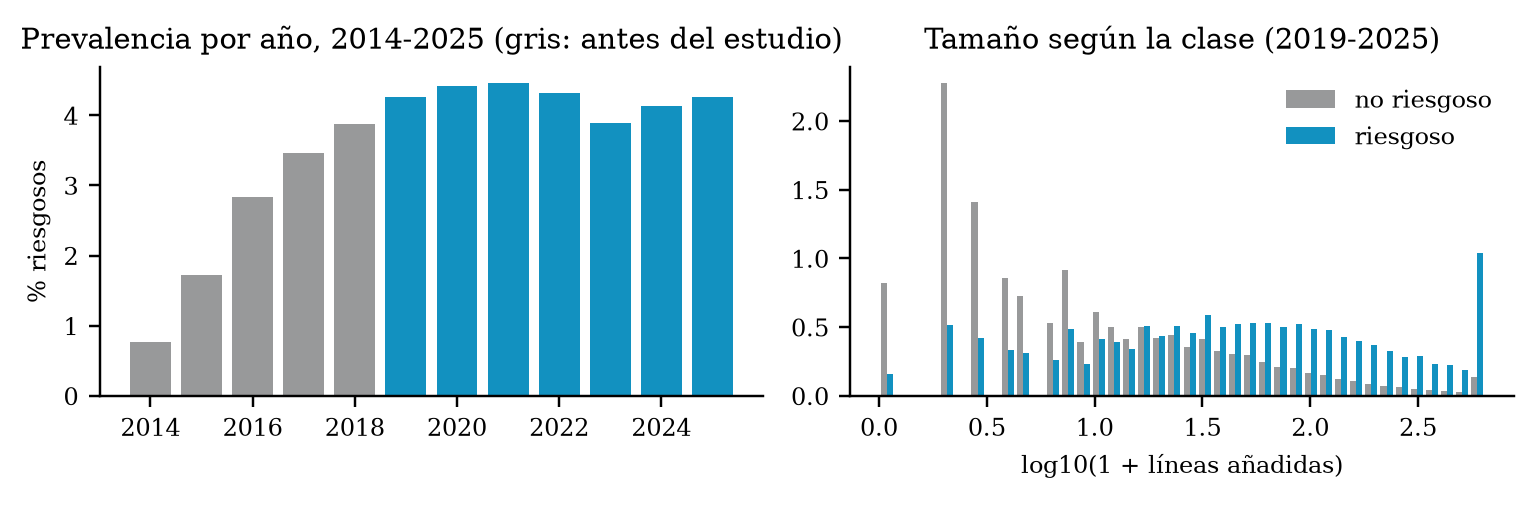
\includegraphics[width=\columnwidth]{../../resultados/e2/prevalencia_y_tamano.png}
\caption{Variable objetivo. Izquierda: balance de clases (prevalencia de riesgosos) por año, 2014--2025; en gris, los años anteriores al estudio. Derecha: distribución de las líneas añadidas por clase en el desarrollo.}
\label{fig:objetivo}
\end{figure}

\begin{figure}[!t]
\centering
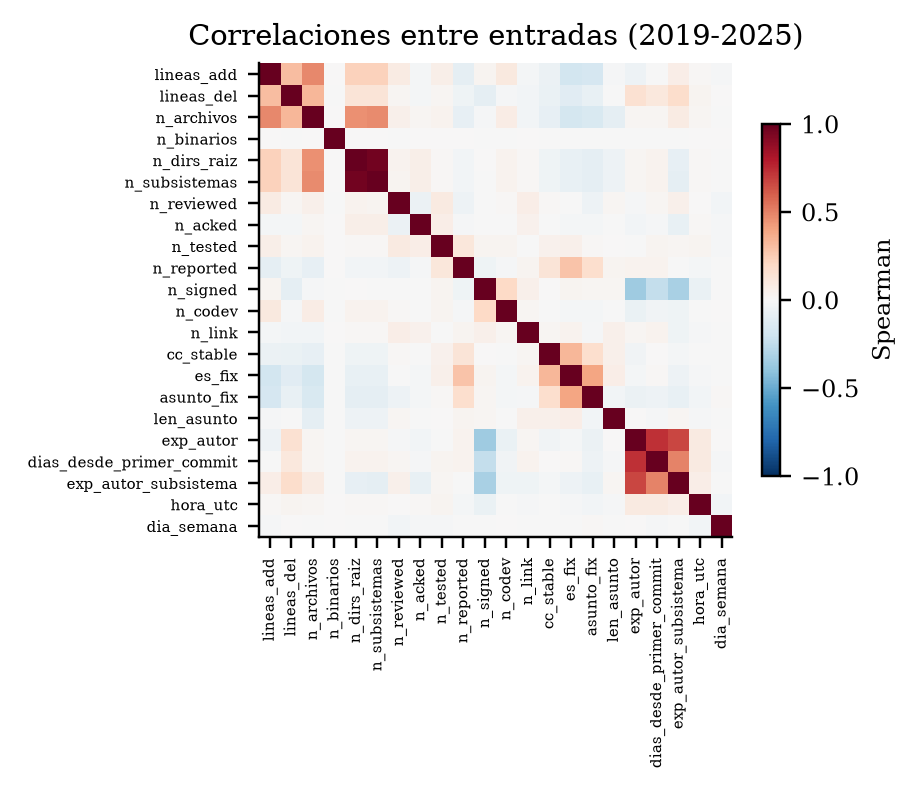
\includegraphics[width=0.92\columnwidth]{../../resultados/e2/correlaciones.png}
\caption{Matriz de correlación de Spearman entre las \cifNVariables{} variables de entrada (desarrollo, 2019--2025).}
\label{fig:corr}
\end{figure}

Los hallazgos del análisis exploratorio orientan las decisiones de preparación y modelado:
\begin{itemize}
\item \textbf{La prevalencia crece hasta 2018 por la adopción de \texttt{Fixes:}} y desde 2019 se estabiliza entre \cifPrevMin{} y \cifPrevMax{} $\rightarrow$ el entrenamiento empieza el 1 de enero de 2019.
\item \textbf{Clases desbalanceadas} (cerca del 4\,\% de positivos) $\rightarrow$ la métrica principal es el AUC-PR \cite{Saito2015} y no se remuestrea, para que la prevalencia de validación sea la real.
\item \textbf{El tamaño es la señal dominante y no es lineal}: la prevalencia pasa de \cifPrevQunoAdd{} en el quintil más pequeño de líneas añadidas a \cifPrevQcincoAdd{} en el más grande, con colas extremas $\rightarrow$ el modelo difuso trabaja sobre la función de distribución empírica y la regresión logística sobre $\log(1+x)$ estandarizado, ambos ajustados solo con el entrenamiento.
\item \textbf{Dos pares casi redundantes}: directorios de primer nivel y subsistemas ($\rho$ = 0,97), y experiencia y antigüedad del autor ($\rho$ = 0,73) $\rightarrow$ el modelo difuso usa solo uno de cada par.
\item \textbf{Deriva en las covariables antes de 2026}: los \texttt{Reviewed-by} por commit suben de \cifReviewedIni{} (2019) a \cifReviewedFin{} (2025) y las correcciones, de \cifFixIni{} a \cifFixFin{} $\rightarrow$ validación por ventanas temporales y no validación cruzada aleatoria.
\end{itemize}

\subsection{Modelos del estudio}
La Tabla~\ref{tab:modelos} define los modelos del estudio y el papel de cada uno. Los modelos se fijaron antes de observar el conjunto de prueba. La regresión logística es el estándar de JIT y es difícil de superar con partición temporal \cite{Kamei2013,Zeng2021}; el \emph{gradient boosting} \cite{Friedman2001} da la cota alta de una caja negra sobre las mismas variables.

\begin{table}[!t]
\caption{Modelos del estudio y su papel}
\label{tab:modelos}
\centering\footnotesize
\begin{tabularx}{\columnwidth}{@{}p{1.35cm} p{1.5cm} Y p{1.15cm}@{}}
\toprule
\cabecera \textbf{Papel} & \textbf{Modelo} & \textbf{Justificación} & \textbf{Parám.}\\
\midrule
Referencia trivial & Clase mayoritaria & Su AUC-PR es la prevalencia: fija el piso & 0\\
Referencia clásica & Regresión logística & Estándar de JIT \cite{Kamei2013,Zeng2021} & 23\\
Referencia clásica fuerte & \emph{Gradient boosting} & Cota alta sin restricción de interpretabilidad \cite{Friedman2001} & $\le$12.600 hojas\\
Propuesto & Difuso-evolutivo & $\le$15 reglas legibles; vértices y reglas ajustados con un AG \cite{Herrera2008,Ishibuchi2001} & \cifGenes{} genes (\cifGenesReales{} reales)\\
Variante sin evolución & Difuso voraz & Mismas reglas iniciales, sin AG: aísla el aporte de la evolución & $\le$15 pesos\\
\bottomrule
\end{tabularx}
\end{table}

Cada variable $x_j$ se lleva a $z_j\in[0,1]$ con su función de distribución empírica, estimada solo con el entrenamiento. Sobre $z_j$ se definen tres términos (bajo, medio y alto) que forman una partición de Ruspini \cite{Ruspini1969} con vértices $a_j<b_j<c_j$. El modelo propuesto se formula como
\begin{equation}
\mu_r(\mathbf{x})=\prod_{(j,t)\in A_r}\mu_{jt}(z_j),\qquad
\hat{y}=s(\mathbf{x})=1-\prod_{r=1}^{R}\bigl(1-w_r\,\mu_r(\mathbf{x})\bigr),
\end{equation}
donde $A_r$ es el conjunto de hasta tres antecedentes (variable $j$, término $t$) de la regla $r$, $\mu_{jt}$ la pertenencia de $z_j$ al término $t$, $w_r\in[0,1]$ el peso de la regla, $R\le15$ el número de reglas activas y $s(\mathbf{x})$ el puntaje de riesgo que ordena los commits (t-norma producto y O probabilístico entre reglas).

El ajuste sigue el enfoque Pittsburgh \cite{Herrera2008,Ishibuchi2001}: cada individuo codifica los $3\times10$ vértices y la base completa de 15 reglas (activación, hasta tres pares variable--término y peso), \cifGenes{} genes en total. La aptitud es el AUC-PR de entrenamiento menos $\lambda$ por antecedente. Los operadores son selección por torneo de 3 con elitismo de 2, cruce uniforme que hereda cada regla completa, y mutación gaussiana de vértices y pesos y aleatoria de antecedentes y términos. El espacio de búsqueda es: población $\{40, 60, 80\}$, generaciones $\{60, 100, 140\}$, reglas $\{5, 10, 15\}$, probabilidad de mutación $\{0{,}05; 0{,}15; 0{,}3\}$, de cruce $\{0{,}7; 0{,}9\}$ y $\lambda\in\{0; 0{,}0005\}$. La variante sin evolución fija los vértices en los cuantiles $(0{,}2; 0{,}5; 0{,}8)$ y elige reglas de 1 o 2 antecedentes de forma voraz; esa misma solución siembra un cuarto de la población inicial del AG.

\textbf{(i) Propiedad de los datos que aprovecha.} El riesgo crece por umbrales con el tamaño y la difusión y se modula con la revisión y la experiencia. Una partición difusa sobre la escala de cuantiles captura esos umbrales sin depender de las colas, y las reglas cortas expresan interacciones que un mantenedor reconoce, como ``si el cambio es grande y toca varios subsistemas''.

\textbf{(ii) Mejores modelos de la matriz y por qué este.} En la matriz, los mejores AUC son de redes profundas y modelos preentrenados sobre el diff \cite{Ni2022}, pero con partición temporal una regresión logística las iguala \cite{Zeng2021}, y ninguno es legible. Se elige un clasificador difuso-evolutivo porque es el vacío identificado y porque el criterio de éxito exige interpretabilidad.

\textbf{(iii) Número de parámetros frente al tamaño.} El individuo tiene \cifGenes{} genes, de los que \cifGenesReales{} son reales. La aptitud se calcula sobre \cifFilasAptitud{} commits (de unos 300.000 en la primera ventana de entrenamiento), más de 500 por gen, así que el riesgo de sobreajuste es bajo; el límite de 15 reglas responde a la interpretabilidad y no al tamaño. La regresión logística (23 parámetros) y el \emph{gradient boosting} (hasta 200 árboles de 63 hojas) también quedan muy por debajo del tamaño del conjunto.

\textbf{(iv) Presupuesto de cómputo.} Cada entrenamiento evalúa hasta \cifEvalAptitud{} individuos (población $\times$ generaciones) sobre una muestra fija de \cifFilasAptitud{} commits. La configuración más cara tardó \cifSegEntrenamiento{} s en un Apple M1 (8 núcleos, 8 GB). El plan prevé \cifNEntrenamientos{} entrenamientos: 14 configuraciones de la búsqueda aleatoria, 9 de sensibilidad y 5 semillas, cada uno en 3 ventanas. Eso suma como cota superior \cifHorasCota{} h en un núcleo, que caben en el presupuesto de una noche y se reducen al paralelizar.

\subsection{Partición y preprocesamiento sin fuga}
\label{sec:particion}
Primero se parten los datos y después se ajusta cualquier transformación. De la tabla publicada (\cifEtresFilas{} filas) se quitan los \cifEtresCensurados{} commits censurados y los \cifEtresPosteriores{} posteriores a julio de 2026; no hay hashes duplicados y las copias por \emph{cherry-pick} se conservan (Sec.~\ref{sec:d1d7}). Quedan \cifEtresDesarrollo{} commits de desarrollo (2019--2025) y \cifEtresPrueba{} de prueba (enero--julio de 2026). De la prueba solo se guardan su tamaño y una huella SHA-256 de sus hashes y etiquetas (\texttt{\cifEtresHuella\ldots}), que la evaluación final debe reproducir; el cuaderno la borra de memoria antes de explorar.

La partición es por bloques temporales con ventana creciente y nunca mezcla commits al azar (Fig.~\ref{fig:particion}, Tabla~\ref{tab:particion}). Para validar el año $V\in\{2023,2024,2025\}$ se entrena desde 2019-01-01 hasta 90 días antes del inicio de $V$. El hueco imita la práctica: al entrenar, las etiquetas de los últimos 90 días todavía no existen. El modelo final se entrena hasta 2025-10-03 y se evalúa una sola vez en la prueba. Como la selección usa etiquetas maduras de todo 2025, la evaluación de 2026 es retrospectiva. Una puesta en marcha el 1 de enero de 2026 requeriría cerrar también la selección con las etiquetas disponibles a esa fecha.

\begin{figure}[!t]
\centering
% Partición temporal: ventana creciente con hueco de 90 días. Escala: 1 año = 0,85 cm desde 2019.
\begin{tikzpicture}[x=0.85cm,y=0.42cm,font=\scriptsize]
  \def\h{0.25}  % hueco de 90 días ~ 0,25 años
  \foreach \y/\lab/\ini in {3/V$_{2023}$/4, 2/V$_{2024}$/5, 1/V$_{2025}$/6}{
    \fill[udazul!70] (0,\y-0.32) rectangle (\ini-\h,\y+0.32);
    \fill[udplata!35] (\ini-\h,\y-0.32) rectangle (\ini,\y+0.32);
    \fill[uddorado!85] (\ini,\y-0.32) rectangle (\ini+1,\y+0.32);
    \node[left,udsable] at (0,\y) {\lab};
  }
  \fill[udazul!70] (0,-0.32) rectangle (7-\h,0.32);
  \fill[udplata!35] (7-\h,-0.32) rectangle (7,0.32);
  \fill[udrojo!80] (7,-0.32) rectangle (7+7/12,0.32);
  \node[left,udsable] at (0,0) {Prueba};
  \draw[udsable] (0,-0.75) -- (8,-0.75);
  \foreach \x/\t in {0/2019,1/2020,2/2021,3/2022,4/2023,5/2024,6/2025,7/2026}
    \draw[udsable] (\x,-0.75) -- ++(0,-0.12) node[below] {\t};
  \node[anchor=west,fill=udazul!70,minimum width=3mm,minimum height=2mm,inner sep=0] (a) at (0,4.2) {};
  \node[anchor=west] at (a.east) {entrenamiento};
  \node[anchor=west,fill=udplata!35,minimum width=3mm,minimum height=2mm,inner sep=0] (b) at (2.2,4.2) {};
  \node[anchor=west] at (b.east) {hueco 90 d};
  \node[anchor=west,fill=uddorado!85,minimum width=3mm,minimum height=2mm,inner sep=0] (c) at (4.1,4.2) {};
  \node[anchor=west] at (c.east) {validación};
  \node[anchor=west,fill=udrojo!80,minimum width=3mm,minimum height=2mm,inner sep=0] (d) at (5.9,4.2) {};
  \node[anchor=west] at (d.east) {prueba};
\end{tikzpicture}

\caption{Partición temporal con ventana creciente y hueco de 90 días. La prueba (enero--julio de 2026) se evalúa una sola vez.}
\label{fig:particion}
\end{figure}

\begin{table}[!t]
\caption{Partición temporal: tamaño y prevalencia de cada bloque}
\label{tab:particion}
\centering\footnotesize
\setlength{\tabcolsep}{3pt}
\begin{tabular}{@{}l c r r r r r@{}}
\toprule
\cabecera & \textbf{Entrenamiento} & \textbf{$n$ entr.} & \textbf{Prev.} & \textbf{$n$ val.} & \textbf{Prev.} & \textbf{Hueco (d)}\\
\midrule
\filas{generado/tabla_particion.tex}
\bottomrule
\end{tabular}
\end{table}

Cada transformación vive dentro de un \texttt{Pipeline} de scikit-learn y se ajusta solo con el entrenamiento de cada ventana (Tabla~\ref{tab:pipeline}). El cuaderno lo comprueba: la media que aprende el escalador coincide con la del entrenamiento y no con la de todo el desarrollo. Ninguna entrada se deriva de commits posteriores: \texttt{dias\_a\_fix}, \texttt{riesgoso} y \texttt{censurado} quedan fuera, y la experiencia del autor solo cuenta sus commits anteriores (no decreciente en el \cifEtresMonotonia{} de los pares consecutivos; el resto son empates de fecha de autor).

\begin{table}[!t]
\caption{Pasos del preprocesamiento}
\label{tab:pipeline}
\centering\footnotesize
\begin{tabularx}{\columnwidth}{@{}p{1.6cm} Y@{}}
\toprule
\cabecera \textbf{Paso} & \textbf{Qué se hace y qué se reporta}\\
\midrule
Limpieza & Se quitan censurados y posteriores a julio de 2026 (cifras arriba); 0 duplicados\\
Faltantes & 0\,\% en las \cifNVariables{} variables; no se imputa\\
Atípicos & Criterio $Q_3+3\,\mathrm{IQR}$ en escala $\log$ (entrenamiento de V$_{2025}$): hasta el \cifEtresAtipMax{} de las filas en los conteos dispersos, como \texttt{n\_acked}, que casi siempre vale 0. Son commits reales, no errores: se conservan y se comprimen con $\log(1+x)$\\
Codificación & No hay categóricas en las entradas (\texttt{subsistema} no entra); hora y día como enteros\\
Escalado & \texttt{StandardScaler} en la regresión logística; el difuso usa la función de distribución empírica (\texttt{QuantileTransformer}); el \emph{boosting} no escala. Todo con el entrenamiento\\
Selección & 22 variables para las referencias y 10 legibles para el difuso, fijadas en el E2\\
Balanceo & No se balancea: el AUC-PR se mide con la prevalencia real y el umbral del MCC se fija en validación \cite{Saito2015}\\
\bottomrule
\end{tabularx}
\end{table}

\subsection{Métricas y pruebas estadísticas}
Se declaran antes de entrenar el modelo propuesto.

\textbf{Principal: AUC-PR} de la clase riesgoso. Con una prevalencia cercana al 4\,\%, el AUC-ROC es engañosamente alto y el AUC-PR refleja la utilidad real de la lista de commits marcados \cite{Saito2015}. Un clasificador sin información obtiene un AUC-PR igual a la prevalencia, así que también se reporta el cociente AUC-PR/prevalencia.

\textbf{Secundarias:} MCC, AUC-ROC, sensibilidad y especificidad. Las que dependen de un umbral usan el que maximiza el MCC en la validación 2025, aplicado tal cual en la prueba. \textbf{Costo:} tiempo de entrenamiento e inferencia y número de parámetros.

\textbf{Incertidumbre y pruebas.} IC del 95\,\% por \emph{bootstrap} (1000 remuestreos) en la prueba y media $\pm$ DE en 5 semillas. McNemar con corrección de continuidad entre el difuso-evolutivo y cada referencia, sobre las mismas observaciones de prueba \cite{Dietterich1998}; Friedman con \emph{post hoc} de Nemenyi sobre los rangos de AUC-PR en las tres ventanas más la prueba \cite{Demsar2006}. $\alpha=0{,}05$. Friedman--Nemenyi se interpreta como exploratorio por el solapamiento del entrenamiento y la selección de hiperparámetros en esas ventanas. Una diferencia sin prueba se reporta como ``diferencia observada''.


%=====================================================================
\section{Experimentación}
\label{sec:experimentacion}

\textbf{Hardware y software.} Apple M1 (8 núcleos, 8 GB de RAM), Python \cifEtresPython{}, pandas \cifEtresPandas{}, NumPy \cifEtresNumpy{} y scikit-learn \cifEtresSklearn{}. El cuaderno lee la copia incluida o descarga los datos del repositorio público \cite{DatosKernel2026} y verifica su SHA-256.

\textbf{Espacios de hiperparámetros.} Se fijan antes de entrenar el modelo propuesto (Tabla~\ref{tab:espacio}). En las referencias, la regresión logística explora $C\in\{0{,}01;\,0{,}1;\,1\}$ y el \emph{gradient boosting} la tasa de aprendizaje $\{0{,}05;\,0{,}1\}\times$ máximo de hojas $\{15, 31, 63\}$, con 200 iteraciones como máximo.

\begin{table}[!t]
\caption{Espacio de hiperparámetros del difuso-evolutivo (arriba, buscados; abajo, fijos)}
\label{tab:espacio}
\centering\footnotesize
\begin{tabularx}{\columnwidth}{@{}l Y@{}}
\toprule
\cabecera \textbf{Hiperparámetro} & \textbf{Valores}\\
\midrule
\filas{../comun/tabla_espacio.tex}
\bottomrule
\end{tabularx}
\end{table}

\textbf{Método de búsqueda.} Las referencias usan rejilla completa. El difuso-evolutivo usa búsqueda aleatoria: 14 de las \cifEtresNConfigs{} configuraciones posibles, cada una evaluada en las tres ventanas con la semilla 11 y elegida por el AUC-PR medio de validación. Después se analiza la sensibilidad en la rejilla máximo de reglas $\times$ probabilidad de mutación ($3\times3$), con el resto fijo en la mejor configuración. Regla de desempate, escrita antes: si dos configuraciones difieren menos que un error estándar, gana la de menos reglas.

\textbf{Semillas.} La búsqueda usa la semilla 11. La configuración elegida y las dos referencias clásicas se entrenan con las 5 semillas (11, 23, 37, 41 y 53) y se reportan media y desviación.

\textbf{Criterios de parada.} El difuso-evolutivo corre un número fijo de generaciones, sin parada temprana, para que el costo sea predecible y comparable entre configuraciones. El \emph{gradient boosting} usa la parada temprana de scikit-learn (10\,\% del entrenamiento como validación interna y 10 iteraciones sin mejora), siempre dentro del entrenamiento. La regresión logística converge con L-BFGS (máximo 3000 iteraciones).

\textbf{Presupuesto de cómputo.} Un entrenamiento del difuso-evolutivo con la configuración máxima tarda \cifSegEntrenamiento{} s (\cifEvalAptitud{} evaluaciones de aptitud sobre \cifFilasAptitud{} commits). Los \cifNEntrenamientos{} entrenamientos previstos (42 de búsqueda, 27 de sensibilidad y 15 de semillas) suman como máximo \cifHorasCota{} h en un núcleo; repartidos en 8 procesos, menos de una hora. Las referencias tardaron \cifEtresMinutos{} min en total (\cifEtresNEntren{} entrenamientos).

\textbf{Prueba del pipeline: referencias en validación.} Las referencias se entrenaron con el mismo pipeline y la misma partición que usará el modelo propuesto (Tabla~\ref{tab:referencias}). La mejor referencia clásica es el \cifEtresMejorClasica{} (\cifEtresConfigGB{}), con AUC-PR medio de \cifEtresValGB{}, frente a \cifEtresValLR{} de la regresión logística y \cifEtresValMay{} de la clase mayoritaria, que iguala la prevalencia. Es la referencia $R$ del criterio de éxito. Entre las ventanas 2023 y 2025 su AUC-PR no cae, sino que sube un \cifEtresCaidaGB{} (la regresión logística, un \cifEtresCaidaLR{}): dentro del desarrollo no se ve degradación. Son cifras de validación: la prueba no interviene en ninguna elección.

\begin{table}[!t]
\caption{Validación de las referencias: AUC-PR por ventana, media y AUC-ROC medio (en negrita, la configuración elegida)}
\label{tab:referencias}
\centering\footnotesize
\setlength{\tabcolsep}{2.5pt}
\begin{tabular}{@{}l l c c c c c@{}}
\toprule
\cabecera \textbf{Modelo} & \textbf{Config.} & \textbf{2023} & \textbf{2024} & \textbf{2025} & \textbf{Media} & \textbf{ROC}\\
\midrule
\filas{generado/tabla_validacion.tex}
\bottomrule
\end{tabular}
\end{table}

\textbf{Reducción de variables por correlación.} La Fig.~\ref{fig:corr} sugiere que el número de subsistemas y el de directorios de primer nivel aportan información similar. Para medir el efecto sobre la mejor referencia clásica, se calculó la correlación de Spearman únicamente en el entrenamiento de cada ventana. Siguiendo el orden de las entradas del cuaderno, se descartó una variable cuando $|\rho|\geq 0{,}85$ con alguna ya conservada. En las tres ventanas salió el número de subsistemas y quedaron 21 de las 22 entradas. Se repitió el ajuste con la misma configuración de \emph{gradient boosting}, semilla y partición que en la Tabla~\ref{tab:referencias}.

Con las 21 entradas, la AUC-PR fue de 0,15840 en 2023, 0,15310 en 2024 y 0,16387 en 2025. Las diferencias frente al modelo completo fueron $+0{,}00149$, $-0{,}00060$ y $+0{,}00115$, respectivamente. El promedio pasó de 0,15778 a 0,15846. Una entrada menos simplifica la representación, pero el cambio de signo en 2024 y el pequeño tamaño de las diferencias aconsejan mantener la referencia original para el contraste previsto. Esta comparación es exploratoria y usa solo datos de desarrollo.


%=====================================================================
\section*{Seguimiento de los comentarios del docente}
{\footnotesize
\begin{tabularx}{\columnwidth}{@{}p{3.3cm} Y@{}}
\toprule
\cabecera \textbf{Comentario} & \textbf{Dónde se atendió}\\
\midrule
\multicolumn{2}{@{}l}{\textit{Entregable 1}}\\
Fecha de ejecución de las consultas & Sec.~II-A: arXiv \fechaConsulta{}, OpenAlex \fechaConsultaOa{}\\
31 frente a 37 estudios citados & Resumen y Sec.~II-A: \nIncluidosCitados{} de los \nTotalIncluidos{} estudios incluidos se citan aquí, más las referencias de método y fuentes del kernel (\nReferencias{} en total); las cifras se calculan a partir del artículo\\
Matriz completa en Excel & Anexo, hoja \emph{matriz\_completa} (\nTotalIncluidos{} trabajos)\\
Algoritmo evolutivo y referencias exactas & Sec.~III-E: codificación, aptitud, operadores y espacio; Tabla~\ref{tab:modelos}\\
Referencia [32] Shehab \emph{et al.} & Con DOI 10.1109/QRS60937.2023.00019\\
PDF o DOI de cada referencia & Anexo, hoja \emph{referencias}: DOI o URL verificada de cada una\\
D3: duplicados por backports & Sec.~III-C: \cifParesCherry{} pares por \emph{cherry-pick}\\
\midrule
\multicolumn{2}{@{}l}{\textit{Entregable 2}}\\
Código de minería y exploración & Cuadernos ejecutados con resultados visibles (Anexo~A)\\
Anexo con diccionario y matriz & Libro Excel del anexo (Tabla~A1 y hojas)\\
Descriptivos y correlaciones & Tabla~\ref{tab:desc} y Fig.~\ref{fig:corr}; completas en el anexo\\
Prevalencia del bloque de prueba & Retirada: la exploración solo usa 2019--2025\\
Parámetros y presupuesto del AG & Tabla~\ref{tab:modelos} y respuestas (iii)--(iv) de la Sec.~III-E\\
Datos con enlace de descarga & Repositorio público con \emph{release} v1.0 y SHA-256 \cite{DatosKernel2026}; el cuaderno lo descarga y lo verifica\\
Pipeline sin fuga (para el E3) & Sec.~\ref{sec:particion}, Tablas~\ref{tab:particion} y \ref{tab:pipeline}, y cuaderno del E3\\
Reducción por correlación & Sec.~IV: comparación de 22 y 21 entradas en tres ventanas temporales.\\
\bottomrule
\end{tabularx}}


\section*{Declaración de uso de inteligencia artificial}
{\footnotesize En las entregas anteriores usé Claude Code (Anthropic, modelos Claude Opus) para la minería de datos, la exploración, la búsqueda bibliográfica y los borradores del informe. Usé Gemini (Google) para revisar la redacción. Contrasté las referencias con sus DOI o URL y comprobé las cifras a partir de los resultados del cuaderno. Para esta entrega usé Codex (OpenAI, GPT-6) como apoyo para revisar el cuaderno, implementar la comparación por correlación y documentar sus resultados. La verificación incluyó la huella del conjunto de datos, la ejecución de las ventanas temporales y la comparación de las métricas del artículo con las salidas del cuaderno.}


% Generado por revision/generar_e1.py 3 en orden de cita; no editar a mano.
\begin{thebibliography}{46}
\bibitem{Mockus2000} A. Mockus and D. M. Weiss, ``Predicting risk of software changes,'' Bell Labs Tech. J., vol. 5, no. 2, pp. 169--180, Apr.--Jun. 2000, doi: \mbox{10.1002/bltj.2229}.
\bibitem{Kamei2013} Y. Kamei, E. Shihab, B. Adams, A. E. Hassan, A. Mockus, A. Sinha, and N. Ubayashi, ``A large-scale empirical study of just-in-time quality assurance,'' IEEE Trans. Softw. Eng., vol. 39, no. 6, pp. 757--773, Jun. 2013, doi: \mbox{10.1109/TSE.2012.70}.
\bibitem{Sliwerski2005} J. Śliwerski, T. Zimmermann, and A. Zeller, ``When do changes induce fixes?'' in Proc. Int. Workshop Mining Softw. Repositories (MSR '05), St. Louis, MO, USA, 2005, pp. 1--5, doi: \mbox{10.1145/1083142.1083147}.
\bibitem{Lyu2024} Y. Lyu, H. J. Kang, R. Widyasari, J. Lawall, and D. Lo, ``Evaluating SZZ implementations: An empirical study on the Linux kernel,'' IEEE Trans. Softw. Eng., vol. 50, no. 9, pp. 2219--2239, Sep. 2024, doi: \mbox{10.1109/TSE.2024.3406718}.
\bibitem{KernelAdd} S. Levin, ``docs: add AI Coding Assistants documentation,'' Linux kernel, commit 78d979db6cef, Jan. 6, 2026. [Online]. Available: \url{https://github.com/torvalds/linux/commit/78d979db6cef}
\bibitem{KernelSimpl} C. Brauner, ``coding-assistants: simplify attribution,'' Linux kernel, commit 816d9992d9ed, Aug. 3, 2026. [Online]. Available: \url{https://github.com/torvalds/linux/commit/816d9992d9ed}
\bibitem{KernelRemove} S. Levin, ``docs: remove Assisted-by references,'' Linux kernel, commit 1e035297ffda, Oct. 14, 2026. [Online]. Available: \url{https://github.com/torvalds/linux/commit/1e035297ffda}
\bibitem{Studer2021} S. Studer, T. B. Bui, C. Drescher, A. Hanuschkin, L. Winkler, S. Peters, and K.-R. M\"uller, ``Towards CRISP-ML(Q): A machine learning process model with quality assurance methodology,'' Mach. Learn. Knowl. Extr., vol. 3, no. 2, pp. 392--413, 2021, doi: 10.3390/make3020020.
\bibitem{MaesBermejo2024} M. Maes Bermejo, J. M. González-Barahona, M. Gallego, and G. Robles, ``A dataset of Linux kernel commits'' (v3), Zenodo, 2024, doi: 10.5281/zenodo.10654193.
\bibitem{Page2021} M. J. Page \emph{et al.}, ``The PRISMA 2020 statement: An updated guideline for reporting systematic reviews,'' BMJ, vol. 372, Art. no. n71, 2021, doi: 10.1136/bmj.n71.
\bibitem{Zeng2021} Z. Zeng, Y. Zhang, H. Zhang, and L. Zhang, ``Deep just-in-time defect prediction: How far are we?'' in Proc. 30th ACM SIGSOFT Int. Symp. Softw. Testing Anal. (ISSTA), Virtual, Denmark, 2021, pp. 427--438, doi: \mbox{10.1145/3460319.3464819}.
\bibitem{Ni2022} C. Ni, W. Wang, K. Yang, X. Xia, K. Liu, and D. Lo, ``The best of both worlds: Integrating semantic features with expert features for defect prediction and localization,'' in Proc. 30th ACM Joint Eur. Softw. Eng. Conf. Symp. Found. Softw. Eng. (ESEC/FSE), Singapore, 2022, pp. 672--683, doi: \mbox{10.1145/3540250.3549165}.
\bibitem{Liu2026} Y. Liu, K. Jabre, R. Abreu, Z. J. Carmichael, V. Murali, A. Patel, J. Ge, W. Sun, C. Zhang, A. Mockus, D. Khavari, P. C. Rigby, and N. Nagappan, ``A preliminary study on explaining risk of code changes using LLM-based prediction models,'' in Proc. 3rd ACM Int. Conf. AI-Powered Softw. (AIware '26), Montreal, QC, Canada, 2026, pp. 259--267, doi: \mbox{10.1145/3805760.3814916}.
\bibitem{JITLine2021} C. Pornprasit and C. K. Tantithamthavorn, ``JITLine: A simpler, better, faster, finer-grained just-in-time defect prediction,'' in Proc. IEEE/ACM 18th Int. Conf. Mining Softw. Repositories (MSR), 2021, pp. 369--379, doi: \mbox{10.1109/MSR52588.2021.00049}.
\bibitem{PyExplainer2021} C. Pornprasit, C. Tantithamthavorn, J. Jiarpakdee, M. Fu, and P. Thongtanunam, ``PyExplainer: Explaining the predictions of just-in-time defect models,'' in Proc. 36th IEEE/ACM Int. Conf. Automated Softw. Eng. (ASE), 2021, pp. 407--418, doi: \mbox{10.1109/ASE51524.2021.9678763}.
\bibitem{Aftab2023} S. Aftab, S. Abbas, T. M. Ghazal, M. Ahmad, H. A. Hamadi, C. Y. Yeun, and M. A. Khan, ``A cloud-based software defect prediction system using data and decision-level machine learning fusion,'' Mathematics, vol. 11, no. 3, Art. no. 632, 2023, doi: \mbox{10.3390/math11030632}.
\bibitem{Dey2025} R. Dey, J. Piri, B. Acharya, P. P. Das, V. C. Gerogiannis, and A. Kanavos, ``A hybrid evolutionary fuzzy ensemble approach for accurate software defect prediction,'' Mathematics, vol. 13, no. 7, Art. no. 1140, 2025, doi: \mbox{10.3390/math13071140}.
\bibitem{McIntosh2018} S. McIntosh and Y. Kamei, ``Are fix-inducing changes a moving target? A longitudinal case study of just-in-time defect prediction,'' IEEE Trans. Softw. Eng., vol. 44, no. 5, pp. 412--428, May 2018, doi: \mbox{10.1109/TSE.2017.2693980}.
\bibitem{Cabral2019} G. G. Cabral, L. L. Minku, E. Shihab, and S. Mujahid, ``Class imbalance evolution and verification latency in just-in-time software defect prediction,'' in Proc. IEEE/ACM 41st Int. Conf. Softw. Eng. (ICSE), Montreal, QC, Canada, 2019, pp. 666--676, doi: \mbox{10.1109/ICSE.2019.00076}.
\bibitem{Olewicki2024} D. Olewicki, S. Habchi, M. Nayrolles, M. Faramarzi, S. Chandar, and B. Adams, ``On the costs and benefits of adopting lifelong learning for software analytics -- Empirical study on brown build and risk prediction,'' in Proc. 46th Int. Conf. Softw. Eng.: Softw. Eng. Pract. (ICSE-SEIP), Lisbon, Portugal, 2024, pp. 275--286, doi: \mbox{10.1145/3639477.3639717}.
\bibitem{Nguyen2025} D. Nguyen, T. Le-Cong, T. H. M. Le, M. A. Babar, and Q.-T. Huynh, ``Toward realistic evaluations of just-in-time vulnerability prediction,'' in Proc. IEEE Int. Conf. Softw. Maint. Evol. (ICSME), Auckland, New Zealand, 2025, pp. 1--10, doi: \mbox{10.1109/ICSME64153.2025.00023}.
\bibitem{Mazloomzadeh2026} I. Mazloomzadeh, M. M. Morovati, and F. Khomh, ``How do AI coding agents contribute to software development? An empirical study of agentic pull requests,'' arXiv:2607.21832, Jul. 2026, doi: \mbox{10.48550/arXiv.2607.21832}.
\bibitem{Herbold2022} S. Herbold, A. Trautsch, F. Trautsch, and B. Ledel, ``Problems with SZZ and features: An empirical study of the state of practice of defect prediction data collection,'' Empir. Softw. Eng., vol. 27, no. 2, Art. no. 42, 2022, doi: \mbox{10.1007/s10664-021-10092-4}.
\bibitem{Falessi2022} D. Falessi, A. Ahluwalia, and M. Di Penta, ``The impact of dormant defects on defect prediction: A study of 19 Apache projects,'' ACM Trans. Softw. Eng. Methodol., vol. 31, no. 1, pp. 1--26, Jan. 2022, doi: \mbox{10.1145/3467895}.
\bibitem{Jiarpakdee2021} J. Jiarpakdee, C. K. Tantithamthavorn, and J. Grundy, ``Practitioners' perceptions of the goals and visual explanations of defect prediction models,'' in Proc. IEEE/ACM 18th Int. Conf. Mining Softw. Repositories (MSR), 2021, pp. 432--443, doi: \mbox{10.1109/MSR52588.2021.00055}.
\bibitem{Sahar2024} H. Sahar, A. A. Bangash, A. Hindle, and D. Barbosa, ``IRJIT: A simple, online, information retrieval approach for just-in-time software defect prediction,'' Empir. Softw. Eng., vol. 29, no. 5, Art. no. 131, 2024, doi: \mbox{10.1007/s10664-024-10514-z}.
\bibitem{Yu2024FoX} J. Yu, M. Fu, A. Ignatiev, C. Tantithamthavorn, and P. Stuckey, ``A formal explainer for just-in-time defect predictions,'' ACM Trans. Softw. Eng. Methodol., vol. 33, no. 7, pp. 1--31, Sep. 2024, doi: \mbox{10.1145/3664809}.
\bibitem{Chen2018MULTI} X. Chen, Y. Zhao, Q. Wang, and Z. Yuan, ``MULTI: Multi-objective effort-aware just-in-time software defect prediction,'' Inf. Softw. Technol., vol. 93, pp. 1--13, Jan. 2018, doi: \mbox{10.1016/j.infsof.2017.08.004}.
\bibitem{Kang2021} J. Kang, S. Kwon, D. Ryu, and J. Baik, ``HASPO: Harmony search-based parameter optimization for just-in-time software defect prediction in maritime software,'' Appl. Sci., vol. 11, no. 5, Art. no. 2002, 2021, doi: \mbox{10.3390/app11052002}.
\bibitem{Mostafa2025} S. Mostafa, S. T. Cynthia, B. Roy, and D. Mondal, ``Feature transformation for improved software bug detection and commit classification,'' J. Syst. Softw., vol. 219, Art. no. 112205, Jan. 2025, doi: \mbox{10.1016/j.jss.2024.112205}.
\bibitem{Chen2025} F. Chen, Y. Ke, X. Liu, and Q. Wei, ``Multi-project just-in-time software defect prediction based on multi-task learning for mobile applications,'' in Proc. IEEE Conf. Softw. Testing, Verification Validation (ICST), 2025, pp. 127--137, doi: \mbox{10.1109/ICST62969.2025.10989004}.
\bibitem{Shehab2023} M. A. Shehab, A. Hamou-Lhadj, and V. S. P. Gunda, ``JITBoost: Boosting just-in-time defect prediction using Boolean combination of classifiers,'' in Proc. IEEE 23rd Int. Conf. Softw. Qual., Rel. Secur. (QRS), 2023, pp. 95--104, doi: \mbox{10.1109/QRS60937.2023.00019}.
\bibitem{Chitsazian2026} Z. Chitsazian, S. Sedighian Kashi, and A. Nikanjam, ``Detecting concept drift in just-in-time software defect prediction using model interpretation,'' Int. J. Syst. Assur. Eng. Manag., vol. 17, no. 9, pp. 2701--2722, 2026, doi: \mbox{10.1007/s13198-025-03122-7}.
\bibitem{Patel2024} H. J. Patel, B. Adams, and A. E. Hassan, ``Post deployment recycling of machine learning models,'' Empir. Softw. Eng., vol. 29, no. 4, Art. no. 100, 2024, doi: \mbox{10.1007/s10664-024-10492-2}.
\bibitem{Tian2026} D. Tian, L. Song, and X. Su, ``Just-in-time quality assurance with assistance of automated defect prediction and code testing,'' ACM Trans. Softw. Eng. Methodol., vol. 35, no. 9, pp. 1--46, 2026, doi: \mbox{10.1145/3779653}.
\bibitem{Song2023} L. Song and L. L. Minku, ``A procedure to continuously evaluate predictive performance of just-in-time software defect prediction models during software development,'' IEEE Trans. Softw. Eng., vol. 49, no. 2, pp. 646--666, Feb. 2023, doi: \mbox{10.1109/TSE.2022.3158831}.
\bibitem{Veras2025} R. C. Veras, G. G. Cabral, and A. L. I. de Oliveira, ``Semantic SZZ: Mitigating the impact of misclassified corrective changes in just-in-time software defect prediction,'' in Proc. IEEE Int. Conf. Syst., Man, Cybern. (SMC), 2025, pp. 769--774, doi: \mbox{10.1109/SMC58881.2025.11342537}.
\bibitem{Gebru2021} T. Gebru, J. Morgenstern, B. Vecchione, J. W. Vaughan, H. Wallach, H. Daum\'e III, and K. Crawford, ``Datasheets for datasets,'' Commun. ACM, vol. 64, no. 12, pp. 86--92, 2021, doi: 10.1145/3458723.
\bibitem{Saito2015} T. Saito and M. Rehmsmeier, ``The precision-recall plot is more informative than the ROC plot when evaluating binary classifiers on imbalanced datasets,'' PLOS ONE, vol. 10, no. 3, Art. no. e0118432, Mar. 2015, doi: \mbox{10.1371/journal.pone.0118432}.
\bibitem{Friedman2001} J. H. Friedman, ``Greedy function approximation: A gradient boosting machine,'' Ann. Statist., vol. 29, no. 5, pp. 1189--1232, Oct. 2001, doi: \mbox{10.1214/aos/1013203451}.
\bibitem{Herrera2008} F. Herrera, ``Genetic fuzzy systems: taxonomy, current research trends and prospects,'' Evol. Intell., vol. 1, no. 1, pp. 27--46, Mar. 2008, doi: \mbox{10.1007/s12065-007-0001-5}.
\bibitem{Ishibuchi2001} H. Ishibuchi, T. Nakashima, and T. Murata, ``Three-objective genetics-based machine learning for linguistic rule extraction,'' Inf. Sci., vol. 136, no. 1--4, pp. 109--133, Aug. 2001, doi: \mbox{10.1016/S0020-0255(01)00144-X}.
\bibitem{Ruspini1969} E. H. Ruspini, ``A new approach to clustering,'' Inf. Control, vol. 15, no. 1, pp. 22--32, Jul. 1969, doi: \mbox{10.1016/S0019-9958(69)90591-9}.
\bibitem{Dietterich1998} T. G. Dietterich, ``Approximate statistical tests for comparing supervised classification learning algorithms,'' Neural Comput., vol. 10, no. 7, pp. 1895--1923, Oct. 1998, doi: \mbox{10.1162/089976698300017197}.
\bibitem{Demsar2006} J. Demšar, ``Statistical comparisons of classifiers over multiple data sets,'' J. Mach. Learn. Res., vol. 7, pp. 1--30, 2006. [Online]. Available: \url{https://jmlr.org/papers/v7/demsar06a.html}
\bibitem{DatosKernel2026} J. F. Rodr\'iguez Galindo, ``Commits del kernel de Linux, 2019--2026, etiquetados por Fixes:,'' v1.0, GitHub, 2026. [Online]. Available: \url{https://github.com/Juferoga/linux-kernel-commits-jit}
\end{thebibliography}


\appendices
\section{Reproducibilidad}
\label{ap:repro}
\begin{itemize}
\item \textbf{Datos:} \url{https://github.com/Juferoga/linux-kernel-commits-jit}, \emph{release} v1.0 (\texttt{kernel-commits-2019-2026.parquet}, 31 MB, SHA-256 \texttt{ac6858f4\ldots45fe9e}) \cite{DatosKernel2026}.
\item \texttt{...-proyecto-e3-cuaderno.ipynb}: cuaderno autocontenido y ejecutado, con salidas visibles. Lee la copia incluida o descarga y verifica los datos, reserva la prueba y reproduce las Tablas~\ref{tab:particion}, \ref{tab:pipeline}, \ref{tab:espacio} y \ref{tab:referencias}. Al ejecutar las celdas, escribe el registro de experimentos (\texttt{registro\_experimentos\_e3.csv}).
\item \texttt{...-proyecto-e2-cuaderno.ipynb}: exploración del Entregable 2 (Tablas~\ref{tab:d1d7} y \ref{tab:desc}, Figs.~\ref{fig:objetivo} y \ref{fig:corr}).
\item Entorno: Python \cifEtresPython{}, pandas \cifEtresPandas{}, NumPy \cifEtresNumpy{} y scikit-learn \cifEtresSklearn{} (\texttt{requirements.txt}). Semillas: 11, 23, 37, 41 y 53.
\end{itemize}

\textbf{Tabla A1. Diccionario de variables.} Está en la hoja \emph{diccionario} del libro de Excel del anexo y en el README del repositorio de datos.


\end{document}
